\begin{figure*}[t]
\centering
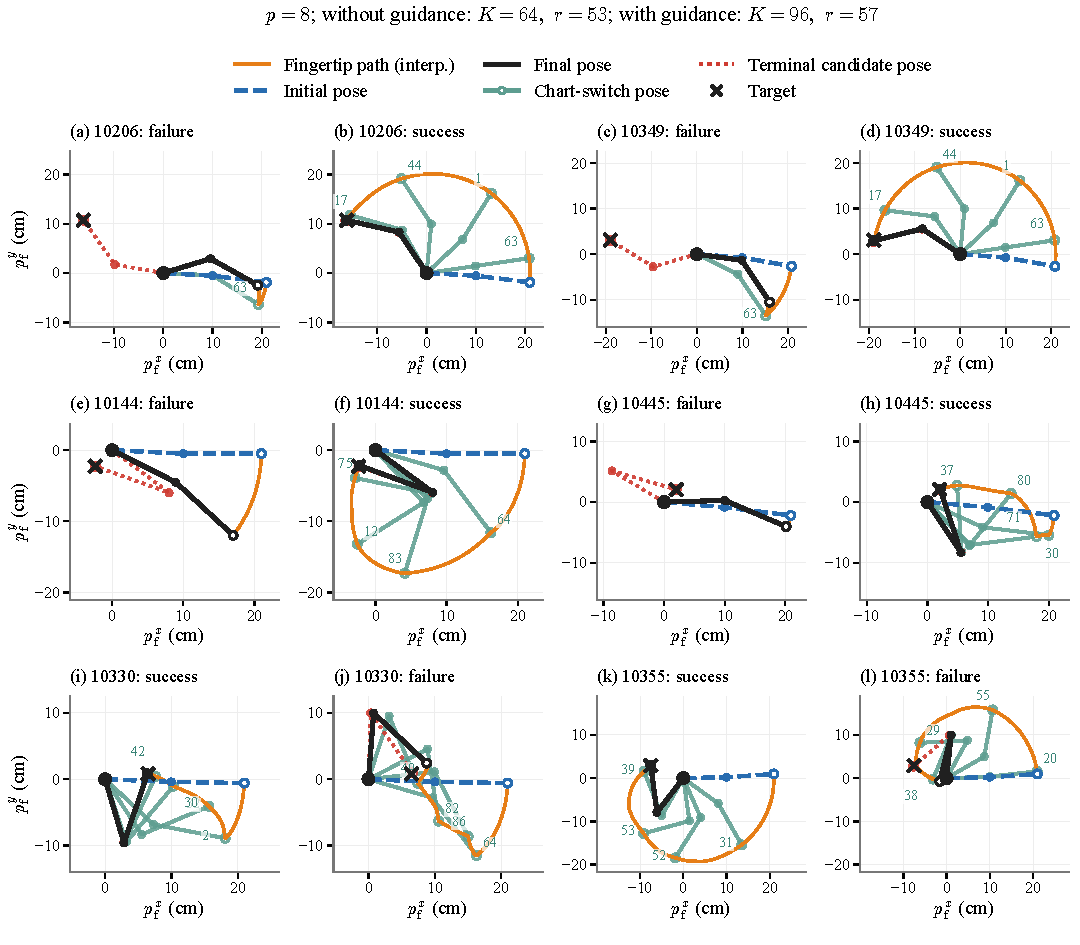
\includegraphics[width=\textwidth]{reacher_p8_guidance_six_seed_pairs.pdf}
\caption{Illustrative paired $p=8$ test rollouts without guidance (first and third columns) and with guidance (second and fourth columns). The top two rows show four failure-to-success pairs; the bottom row shows two success-to-failure pairs. Each adjacent pair shares its initial state and target. The unguided and guided configurations use separately tuned atlases, $(K,r)=(64,53)$ and $(96,57)$, respectively; this is not a guidance-only ablation. Orange curves show interpolated measured fingertip paths; green arms show selected measured chart-switch poses labeled by chart ID. Red dotted arms show the offline pose of the final selected terminal candidate. Only a subset of chart-switch poses is shown for clarity. These are selected examples from 35 failure-to-success and 14 success-to-failure pairs among 500 test seeds.}
\label{fig:reacher-guidance-recovery}
\end{figure*}
